\paragraph*{Breakdown of the product-state description.}
We first take the parameters of a Zeeman-polarized dot embedded in a short
BCS ring ($t=2$, $\Delta=0.6$, $L=11$, $\epsilon_{d\uparrow}=-0.3$,
$\epsilon_{d\downarrow}=3.7$, $t_J=0.5$, $\hbar\omega=0.02$). The
self-consistent product state predicts a current-carrying phase for
$g\gtrsim0.75$, with $\langle a^\dagger a\rangle\simeq1$--$1.4$ and
$|\langle I\rangle|\approx0.02$ [Fig.~\ref{fig:notebook}]. DMRG shows that this
phase is an artefact. The exact ground-state energy decreases monotonically with
$g$ and lies below the MF energy by up to $1.9\hbar\omega$ \TODO{update with
DMRG g=1.2}. The gap to the first excited state stays a sizeable fraction of
$\hbar\omega$ ($E_1-E_0=0.34\hbar\omega$ at $g=1.2$). The linear response to the
seed flux $\varphi_{\rm cl}=10^{-3}$ remains $\langle I\rangle\lesssim
4\times10^{-4}$, i.e.\ two orders of magnitude below the MF value. DMRG and
the adiabatic theory~\eqref{eq:BO} agree to within
$\lesssim2\%$ of $\hbar\omega$ in energy and to $<1\%$ in $E_1-E_0$.
The residual difference is the non-adiabatic (diagonal Born--Oppenheimer)
correction $\sim g^2\hbar\omega\,\hbar\omega/E_A$.

Two effects make the product state fail. (i) It is not gauge invariant~\cite{Li2020,Dmytruk2021}: with the full
Peierls phase on one bond, it renormalizes that bond by
$|\langle D\rangle|<1$ and so loses phase-\emph{independent} kinetic energy,
which the exact state recovers by following the flux adiabatically. (ii) Here
$E_J\simeq\hbar\omega$. The Landau free energy does develop a double well
for $g>0.58$, but its depth is below the zero-point energy, and the flux
distribution $P(X)$ stays essentially unimodal. A further subtlety
concerns ring size: since $L\lesssim\xi$, $E(\varphi)$ of this ring is dominated by the
single-electron harmonic, $E_1=2.1\times10^{-2}\gg E_2=2.0\times10^{-3}$
[Fig.~\ref{fig:junctions}(a)]. The instability would then be one of the normal
$h/e$ persistent current rather than of the Josephson junction. To isolate
Josephson physics we use rings with $L\gg\xi$ below
($t=1$, $\Delta=1$, $L=14$, giving $|E_1/E_2|\lesssim10^{-2}$).

\paragraph*{Half-flux-biased junction.}
For an ordinary weak link ($t_J=0.5$, $E_2=-0.056\,t$, Andreev gap
$0.77\,t$) biased by $\Phi_0/2$, Fig.~\ref{fig:halfflux} shows the full
DMRG solution at $E_J/\hbar\omega=10$ as a function of $\beta$.
\TODO{fill: DMRG current jumps to $|\langle I\rangle|\simeq I^\star$ at
$\beta\simeq1$, follows BO within ..., MF ...}
The flux distribution extracted from the photon reduced density matrix
evolves from a Gaussian centred at zero to a single displaced peak at
$\pm\Phi^\star$. The sign is fixed by the residual odd harmonic
$E_1=-5.4\times10^{-4}$, which tilts the double well by
$2|E_1|\sin\varphi^\star\approx10^{-3}t\approx0.2\hbar\omega$.
This tilt sets the splitting $E_1-E_0$ for $\beta>1.2$ in DMRG and BO alike. Without it,
$\delta/\hbar\omega$ would drop below $10^{-6}$ at $\beta=2$. The external-bias
route thus provides a current-carrying state whose direction is \emph{selected}
rather than spontaneously chosen. Its residual symmetry breaking is
$\propto e^{-L/\xi}$ for a homogeneous ring, but in practice it is limited
by the flux offset $\delta\Phi$.

\paragraph*{Interaction-driven $\pi$ junction without external flux.}
We now replace the weak link by an Anderson impurity at particle--hole
symmetry ($\epsilon_d=-U/2$, $t_J=0.5$) and set $\varphi_{\rm cl}=0$.
DMRG in the even and odd fermion-parity sectors
[Fig.~\ref{fig:junctions}(b,c)] gives the $0$--$\pi$ transition known for magnetic quantum dots~\cite{GlazmanMatveev1989,SpivakKivelson1991,Vecino2003,Karrasch2008,vanDam2006,Cleuziou2006,Delagrange2015}. For
$U<U_c\simeq0.9\,t$ the singlet (even) state is the ground state at $\varphi=0$
and the junction is a $0$-junction. For $U>U_c$ the Kramers doublet (odd sector)
is the ground state at all phases, and $E(\varphi)$ has its \emph{minimum} at the
Cooper-pair phase $\pi$. At $U=2t$ we find $E_2=+7.39\times10^{-3}t$, with
$|E_1|,|E_4|<10^{-4}t$: a pure $\pi$ junction, indistinguishable after
normalization from the half-flux-biased weak link [Fig.~\ref{fig:junctions}(a)].
The $\pi$ coupling decreases monotonically with $U$ ($E_2\propto U^{-1.3}$ for $4t\le U\le10t$), as expected for
cotunnelling through the singly occupied level.

Coupling this junction to the mode [Fig.~\ref{fig:udot}] gives the
transition without any static flux. Here $H_{\rm ring}$ is real and
$\langle I\rangle=0$ in every eigenstate, so the order is diagnosed by the
two lowest states. The splitting $\delta=E_1-E_0$ collapses and the
flux operator projected onto the quasi-degenerate doublet acquires the eigenvalues
$\pm\Phi^\star$. \TODO{fill DMRG numbers: at $E_J/\hbar\omega=10$, $\delta/\hbar\omega=$
... at $\beta=2$ and ... at $\beta=3$; $\Phi^\star$ ...}. In the photon-number basis
the DMRG ground state is a cat state: $P(\Phi)$ is bimodal with peaks at
$\pm\Phi^\star$, whose separation tracks the classical minimum. With
increasing $E_J/\hbar\omega$ the crossover sharpens into a pitchfork at
$\beta=1$ and $\delta$ vanishes exponentially [Fig.~\ref{fig:udot}(b)]. The
residual $\delta$ is the macroscopic tunnelling of a persistent current. Because
it is protected by time-reversal symmetry, it is the only
energy scale separating the two current directions. Each current state is
additionally Kramers degenerate in the spin of the dot. The low-energy manifold is
therefore a fourfold multiplet $\{\sigma=\uparrow,\downarrow\}\otimes\{\circlearrowright,\circlearrowleft\}$,
split only by $\delta$.

\paragraph*{Experimental scales.}
The two control parameters are
$\beta=2\pi L I_c/\Phi_0$ and $E_J/\hbar\omega$, related by
$\beta=2\pi(Z/R_Q)(E_J/\hbar\omega)$, with $E_J/h\simeq0.5\,{\rm GHz}\times I_c[{\rm nA}]$.
Three classes of $\pi$ elements span the phase diagram
[Fig.~\ref{fig:overview}(b)]:
(i) SFS junctions ($I_c\sim1$--$100\,\mu$A) reach $\beta>1$ with geometric
inductances of a few to a few hundred pH and $E_J/\hbar\omega\sim10^2$--$10^4$.
This is the classical limit, where the half-flux state is fully polarized,
consistent with the spontaneous currents observed in SFS
and $d$-wave $\pi$ loops~\cite{Tsuei2000,Ryazanov2001,Bauer2004}.
(ii) Quantum-dot $\pi$ junctions in the doublet regime
($I_c^\pi\sim0.1$--$10$\,nA) require $L\sim0.03$--$3\,\mu$H, i.e.\ superinductances
(Josephson-junction arrays, granular Al) as in fluxonium circuits~\cite{Manucharyan2009,Grunhaupt2019}; this is the $\pi$-qubit regime of Refs.~\cite{Ioffe1999,Yamashita2005,Feofanov2010}. These give
$E_J/\hbar\omega\sim1$: the ground state is the
cat state $(|{\circlearrowright}\rangle+|{\circlearrowleft}\rangle)/\sqrt2$ with
$\delta\sim0.1\hbar\omega$, and the transition appears as a dip in the
$|0\rangle\to|1\rangle$ frequency and a jump in the transition matrix element
$\langle0|\Phi|1\rangle$, accessible in two-tone spectroscopy.
(iii) Multichannel or gate-tunable $\pi$ junctions with
$I_c\sim50$--$200$\,nA in a high-kinetic-inductance loop ($L\sim2$--$10$\,nH,
$\omega/2\pi\sim2$--$5$\,GHz) give $\beta\sim1$--$3$ and $E_J/\hbar\omega\sim10$--$30$.
This is the regime of Figs.~\ref{fig:halfflux} and~\ref{fig:udot}: a well-defined
current-carrying state whose residual tunnelling $\delta/\hbar\omega\sim10^{-4}$--$10^{-8}$
remains a measurable macroscopic-quantum-tunnelling signature.
In the externally biased realization, the half-flux bias must be stable to
$|\delta\Phi|\ll\delta/2I^\star$, i.e.\ $\lesssim10^{-6}\Phi_0$ for the parameters above.
The interaction-driven realization has no such requirement.


% ------------------------------------------------------------------ figures
\begin{figure*}
  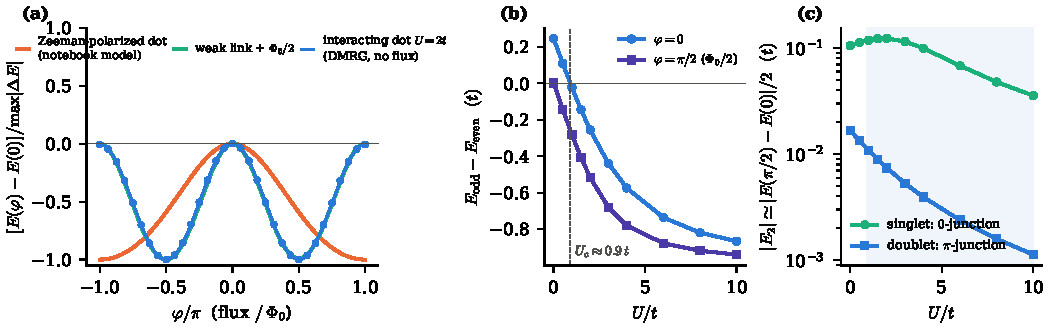
\includegraphics[width=\textwidth]{../figs/fig_junctions.pdf}
  \caption{\label{fig:junctions}%
  (a) Normalized ground-state energy of the loop versus the electron phase
  $\varphi$ (flux in units of $h/2e$) for three junctions:
  Zeeman-polarized dot in a short ring (dominated by the single-electron
  harmonic $\cos\varphi$), an ordinary weak link biased by $\Phi_0/2$, and an
  interacting dot at $U=2t$ without any bias (DMRG, symbols; line: cosine fit).
  (b) Parity competition $E_{\rm odd}-E_{\rm even}$ of the interacting-dot
  ring at $\varphi=0$ and $\varphi=\pi/2$ (DMRG, $L=14$, $\Delta=t$, $t_J=0.5t$).
  (c) Josephson energy $|E_2|$ in the singlet ($0$) and doublet ($\pi$)
  sectors. Shading: doublet ground state.}
\end{figure*}

\begin{figure}
  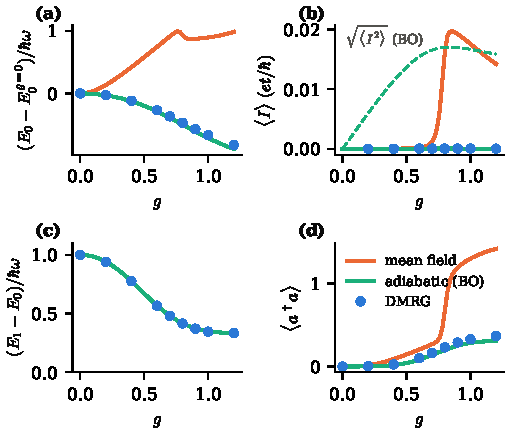
\includegraphics[width=\columnwidth]{../figs/fig_notebook_model.pdf}
  \caption{\label{fig:notebook}%
  Short ring with a Zeeman-polarized dot ($\hbar\omega=0.02$,
  $\varphi_{\rm cl}=10^{-3}$): mean field (MF, orange), adiabatic
  theory~\eqref{eq:BO} (green), and DMRG (symbols).
  (a) Ground-state energy, (b) current (dashed: rms current of the BO
  ground state), (c) gap to the first excited state, (d) photon number.}
\end{figure}

\begin{figure*}
  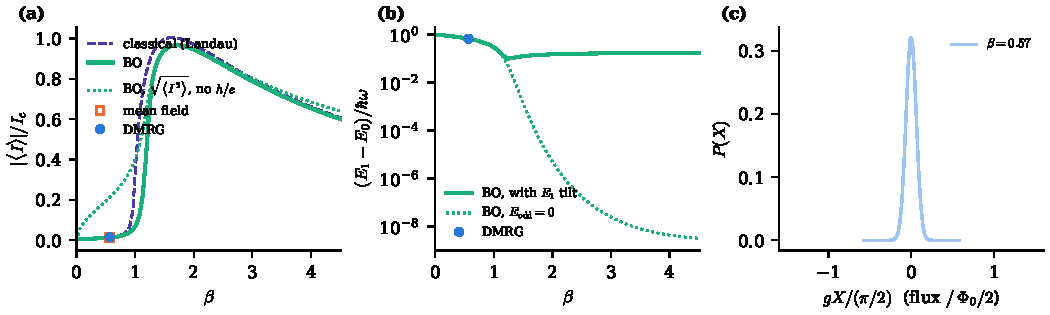
\includegraphics[width=\textwidth]{../figs/fig_weaklink_halfflux.pdf}
  \caption{\label{fig:halfflux}%
  Weak-link loop biased by $\Phi_0/2$, $E_J/\hbar\omega=10$.
  (a) Persistent current versus $\beta$: DMRG (circles), MF (squares), adiabatic
  theory with (solid) and without (dotted) the odd harmonics, classical
  Landau theory (dashed). (b) Splitting of the two lowest levels.
  (c) Flux distribution of the DMRG ground state, obtained from the photon reduced
  density matrix.}
\end{figure*}

\begin{figure*}
  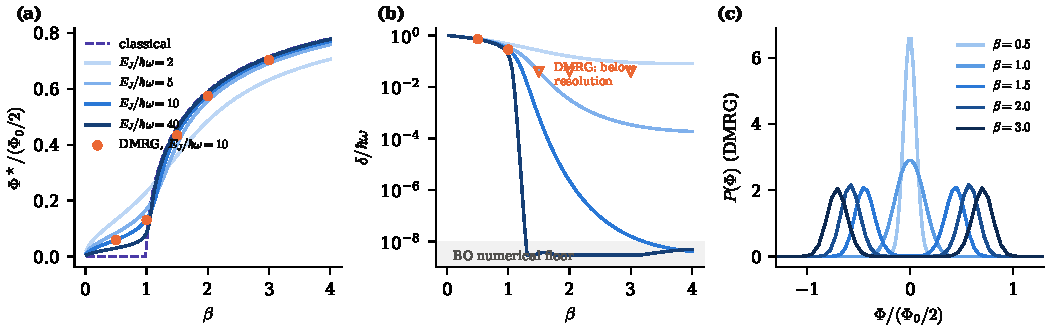
\includegraphics[width=\textwidth]{../figs/fig_udot_cavity.pdf}
  \caption{\label{fig:udot}%
  Interaction-driven $\pi$ loop ($U=2t$, no external flux).
  (a) Flux of the condensate $\Phi^\star$ (eigenvalue of the flux projected on the two
  lowest states) versus $\beta$ for increasing $E_J/\hbar\omega$ (lines: adiabatic
  theory with the DMRG $E(\varphi)$; circles: full DMRG at $E_J/\hbar\omega=10$;
  dashed: classical). (b) Tunnel splitting $\delta$ between the two
  current-carrying states. (c) Flux distribution of the DMRG ground state
  (a cat state for $\beta>1$).}
\end{figure*}
